\documentclass[a4paper]{article}
\usepackage[a4paper,margin=0mm]{geometry}
\usepackage{fontspec}
\usepackage{unicode-math}
\usepackage{tikz}
\usepackage[table]{xcolor}
\usepackage[absolute]{textpos}
\usepackage{enumitem}
\usepackage{array}
\usepackage{multirow}

\setmainfont{Libertinus Serif}
\setsansfont{Libertinus Sans}
\setmathfont{Libertinus Math}
\newfontfamily\trackedsans{Libertinus Sans}[LetterSpace=8.0]

\definecolor{accent}{HTML}{F46530}
\definecolor{badge}{HTML}{FFBDA5}
\definecolor{ink}{HTML}{2A2E30}

\setlength{\TPHorizModule}{1mm}
\setlength{\TPVertModule}{1mm}
\setlength{\parindent}{0pt}
\pagestyle{empty}

\newcommand{\LCOL}{16mm}
\newcommand{\RCOL}{111mm}
\newcommand{\COLW}{83mm}

\newcommand{\topicheader}[2]{%
\begin{textblock*}{194mm}(16mm,10mm)
\begin{tikzpicture}
\node[fill=accent,text=white,font=\sffamily\bfseries\fontsize{13}{13}\selectfont,
      minimum width=9mm,minimum height=9mm,inner sep=0pt] at (4.5mm,-4.5mm) {#1};
\node[font=\sffamily\bfseries\fontsize{15}{16}\selectfont,text=ink,anchor=west] at (12mm,-4.5mm) {#2};
\end{tikzpicture}
\end{textblock*}
\begin{textblock*}{194mm}(16mm,22.5mm)

\begin{tikzpicture}
\fill[accent] (0,0) rectangle (194mm,0.5mm);
\end{tikzpicture}
\end{textblock*}
}

\newcommand{\pagefooter}[1]{%
\begin{textblock*}{194mm}(8mm,286.41mm)
  
\begin{tikzpicture}
    \fill[accent] (0,0) rectangle (194mm,0.6mm);
  \end{tikzpicture}
\end{textblock*}
\begin{textblock*}{63.59mm}(8mm,288.27mm)
  {\sffamily\bfseries\color{accent}\fontsize{13}{16}\selectfont SAT 1200+}
\end{textblock*}
\begin{textblock*}{10mm}(188mm,288.27mm)
  \centering{\sffamily\color{accent}\fontsize{14}{16}\selectfont #1}
\end{textblock*}
}

\newcommand{\colrule}[2]{%
\begin{textblock*}{1mm}(105mm,#1mm)
\begin{tikzpicture}
\draw[black!65,line width=0.5pt] (0,0) -- (0,#2mm);
\end{tikzpicture}
\end{textblock*}
}

\newcommand{\setkicker}[2]{%
{\sffamily\bfseries\fontsize{12}{14}\selectfont #1.}\ {\itshape\fontsize{11}{14}\selectfont\color{black!75} #2}\par\vspace{2mm}%
}

\setlength{\fboxsep}{1.4pt}
\setlength{\fboxrule}{0.5pt}
\newcommand{\pnum}[1]{\fcolorbox{ink}{white}{\sffamily\bfseries\fontsize{8}{8}\selectfont #1}~}

\newcommand{\qrbox}[1]{%
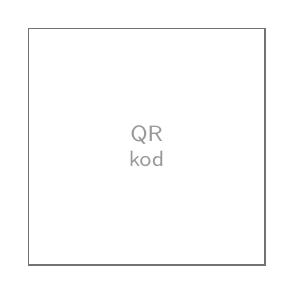
\begin{tikzpicture}
\draw[black!55,line width=0.6pt] (0,0) rectangle (30mm,30mm);
\node[black!40,font=\sffamily\fontsize{8}{9}\selectfont,align=center] at (15mm,15mm) {QR\\kod};
\end{tikzpicture}\\[1.5mm]
{\sffamily\fontsize{9}{11}\selectfont\color{black!70} #1}%
}

% ---- SAT-style multiple-choice question block: #1=number #2=stem #3-6=choices A-D ----
\newcommand{\satq}[6]{%
\noindent\pnum{#1} #2\\[2mm]
\hspace*{7mm}\begin{tabular}{@{}p{32mm}p{32mm}@{}}
(A) #3 & (B) #4 \\[2.5mm]
(C) #5 & (D) #6 \\
\end{tabular}\\[7mm]%
}

\arrayrulecolor{accent}
\setlength{\arrayrulewidth}{0.7pt}
\renewcommand{\arraystretch}{1.35}
\newcommand{\anstitle}[1]{{\sffamily\bfseries\color{accent}\fontsize{11}{13}\selectfont #1}\\[1.3mm]}

\begin{document}

% ================= PAGE 1: Set 1 | Set 2 =================
\topicheader{6}{BIR O'ZGARUVCHILI TENGLAMALAR}
\pagefooter{48}
\colrule{32}{238}
\mbox{}%

\begin{textblock*}{\COLW}(\LCOL,32mm)
{\fontsize{12}{15}\selectfont
\setkicker{1-to'plam}{Bir qadamli tenglamalar -- asosiy amalni teskarisi bilan bajaring.}

\noindent\pnum{1} $x+7=12$\\[22mm]
\noindent\pnum{2} $x-9=4$\\[22mm]
\noindent\pnum{3} $5x=35$\\[22mm]
\noindent\pnum{4} $\dfrac{x}{4}=6$\\[22mm]
\noindent\pnum{5} $x-(-3)=10$\\[22mm]
\noindent\pnum{6} $-3x=21$\\[22mm]
\noindent\pnum{7} $x+15=8$\\[22mm]
\noindent\pnum{8} $\dfrac{x}{-5}=-6$
}
\end{textblock*}

\begin{textblock*}{\COLW}(\RCOL,32mm)
{\fontsize{12}{15}\selectfont
\setkicker{2-to'plam}{Ikki qadamli tenglamalar -- qo'shish/ayirishdan so'ng ko'paytirish/bo'lish.}

\noindent\pnum{1} $2x+3=11$\\[22mm]
\noindent\pnum{2} $3x-5=10$\\[22mm]
\noindent\pnum{3} $\dfrac{x}{2}+4=9$\\[22mm]
\noindent\pnum{4} $5-2x=1$\\[22mm]
\noindent\pnum{5} $4x+7=-5$\\[22mm]
\noindent\pnum{6} $-3x-2=10$\\[22mm]
\noindent\pnum{7} $\dfrac{x}{3}-1=-4$\\[22mm]
\noindent\pnum{8} $7-\dfrac{x}{2}=3$
}
\end{textblock*}

\clearpage

% ================= PAGE 2: Set 3 | Set 4 =================
\topicheader{6}{BIR O'ZGARUVCHILI TENGLAMALAR}
\pagefooter{49}
\colrule{32}{238}
\mbox{}%

\begin{textblock*}{\COLW}(\LCOL,32mm)
{\fontsize{12}{15}\selectfont
\setkicker{3-to'plam}{Qavsni ochish va o'xshash hadlarni birlashtirish.}

\noindent\pnum{1} $3(x+2)=15$\\[22mm]
\noindent\pnum{2} $2(x-4)+5=7$\\[22mm]
\noindent\pnum{3} $4x+2x-3=15$\\[22mm]
\noindent\pnum{4} $-2(x+3)=10$\\[22mm]
\noindent\pnum{5} $3(2x-1)-2x=13$\\[22mm]
\noindent\pnum{6} $6-3(x-2)=0$\\[22mm]
\noindent\pnum{7} $2(3x+1)-(x-5)=22$\\[22mm]
\noindent\pnum{8} $-4(x-1)+2x=-2$
}
\end{textblock*}

\begin{textblock*}{\COLW}(\RCOL,32mm)
{\fontsize{12}{15}\selectfont
\setkicker{4-to'plam}{O'zgaruvchi ikkala tomonda -- avval bir tomonga yig'ing.}

\noindent\pnum{1} $3x+5=x+13$\\[22mm]
\noindent\pnum{2} $5x-2=2x+7$\\[22mm]
\noindent\pnum{3} $4x+1=2x-9$\\[22mm]
\noindent\pnum{4} $7-x=2x+1$\\[22mm]
\noindent\pnum{5} $2(x+3)=x+10$\\[22mm]
\noindent\pnum{6} $3x-4=5(x-2)$\\[22mm]
\noindent\pnum{7} $x+8=3x-2$\\[22mm]
\noindent\pnum{8} $6-2x=4x-18$
}
\end{textblock*}

\clearpage

% ================= PAGE 3: Set 5 (SAT-style, derived expression) | Set 6 (spot the error) =================
\topicheader{6}{BIR O'ZGARUVCHILI TENGLAMALAR}
\pagefooter{50}
\colrule{32}{238}
\mbox{}%

\begin{textblock*}{\COLW}(\LCOL,32mm)
{\fontsize{11}{14}\selectfont
\setkicker{5-to'plam}{Aralash, SAT uslubida -- ba'zilari $x$ emas, hosila ifodani so'raydi. Diqqat bilan o'qing.}

\noindent\pnum{1} $2x+5=17$. $x+3$ ning qiymati nechaga teng?\\[14mm]
\noindent\pnum{2} $3(x-2)=2x+1$. $2x$ ning qiymati nechaga teng?\\[14mm]
\noindent\pnum{3} $\dfrac{x}{2}+3=9$. $3x$ ning qiymati nechaga teng?\\[14mm]
\noindent\pnum{4} $4x-7=x+8$. $x-1$ ning qiymati nechaga teng?\\[14mm]
\noindent\pnum{5} $2(2x+1)-3=15$. $x$ ning qiymati nechaga teng?\\[14mm]
\noindent\pnum{6} $5x+2=3x+12$. $5x$ ning qiymati nechaga teng?\\[14mm]
\noindent\pnum{7} $6-x=2x-6$. $x+4$ ning qiymati nechaga teng?\\[14mm]
\noindent\pnum{8} $3(x-1)=x+5$. $2x-1$ ning qiymati nechaga teng?
}
\end{textblock*}

\begin{textblock*}{\COLW}(\RCOL,32mm)
{\fontsize{11}{14}\selectfont
\setkicker{6-to'plam}{Xatoni toping -- buzilgan qadamni ayting, to'g'ri javobni bering.}

\noindent\pnum{1} $x-5=12$ ifodasida ko'rsatilgan yechimda xato bor:\\[1mm]
\hspace*{7mm}\textit{``1-qadam: ikkala tomonga 5 qo'shiladi: $x=12$.''}\\[2mm]
\hspace*{7mm}Xato va to'g'ri javob: \makebox[52mm]{\dotfill}\\[8mm]

\noindent\pnum{2} $2x-5=9$ ifodasida ko'rsatilgan yechimda xato bor:\\[1mm]
\hspace*{7mm}\textit{``1-qadam: $2x=9-5=4$.''}\\[2mm]
\hspace*{7mm}Xato va to'g'ri javob: \makebox[52mm]{\dotfill}\\[8mm]

\noindent\pnum{3} $-2(x-3)=10$ ifodasida ko'rsatilgan yechimda xato bor:\\[1mm]
\hspace*{7mm}\textit{``1-qadam: $-2x-6=10$.''}\\[2mm]
\hspace*{7mm}Xato va to'g'ri javob: \makebox[52mm]{\dotfill}\\[8mm]

\noindent\pnum{4} $3x+5=20$ ifodasida ko'rsatilgan yechimda xato bor:\\[1mm]
\hspace*{7mm}\textit{``1-qadam: $8x=20$, shuning uchun $x=2.5$.''}\\[2mm]
\hspace*{7mm}Xato va to'g'ri javob: \makebox[52mm]{\dotfill}\\[8mm]

\noindent\pnum{5} $2x+1=11$ (savolda $3x$ so'ralgan) ifodasida ko'rsatilgan yechimda xato bor:\\[1mm]
\hspace*{7mm}\textit{``$x=5$, javob: 5.''}\\[2mm]
\hspace*{7mm}Xato va to'g'ri javob: \makebox[52mm]{\dotfill}
}
\end{textblock*}

\clearpage

% ================= PAGE 4: Set 7 (bonus, left) + Set 8 pt.1 (right) -- no dead column =================
\topicheader{6}{BIR O'ZGARUVCHILI TENGLAMALAR}
\pagefooter{51}
\colrule{32}{238}
\mbox{}%

\begin{textblock*}{\COLW}(\LCOL,32mm)
{\fontsize{12}{15}\selectfont
\setkicker{7-to'plam}{Bonus / qiyin -- kasr va qavslar birgalikda, har biriga taxminan 90 soniya.}

\noindent\pnum{1} $\dfrac{x+3}{2}=7$\\[26mm]
\noindent\pnum{2} $\dfrac{3(x-1)}{2}=6$\\[26mm]
\noindent\pnum{3} $2(x+1)-3(x-2)=10$\\[26mm]
\noindent\pnum{4} $\dfrac{2x-1}{3}+1=4$\\[26mm]
\noindent\pnum{5} $4(x-2)=2(x+3)-6$
}
\end{textblock*}

\begin{textblock*}{\COLW}(\RCOL,32mm)
{\fontsize{10.5}{13}\selectfont
\setkicker{8-to'plam}{SAT'da qanday uchraydi -- haqiqiy kontekstdagi tenglamalar.}

\satq{1}{Aziz yoshi singlisining yoshidan ikki baravar ortig'idan 5 yosh katta. Agar Aziz 17 yoshda bo'lsa, singlisi necha yoshda?}{11}{6}{12}{22}
\satq{2}{Avtomobil to'xtash joyi uchun boshlang'ich to'lov \$15, har bir qo'shimcha soat uchun esa \$4 olinadi. Agar jami to'lov \$47 bo'lsa, necha soat to'xtalgan?}{6}{11}{8}{32}
\satq{3}{$4x-7=21$ tenglamada $x$ ning qiymati nechaga teng?}{7}{3}{5}{9}
\satq{4}{$3(x+4)=30$ tenglamada $x$ ning qiymati nechaga teng?}{4}{8}{14}{6}
\satq{5}{Ikki firma narxlari: A firma -- \$20 + har bir mahsulot uchun \$3; B firma -- \$8 + har bir mahsulot uchun \$5. Nechta mahsulot sotib olinganda ikkala firma narxi teng bo'ladi?}{6}{4}{8}{12}
\satq{6}{$5x+3=28$ bo'lsa, $2x$ ning qiymati nechaga teng?}{5}{14}{10}{25}
}
\end{textblock*}

\clearpage

% ================= PAGE 5: Set 8 pt.2 (continues directly, no title page of its own) =================
\topicheader{6}{BIR O'ZGARUVCHILI TENGLAMALAR}
\pagefooter{52}
\colrule{32}{238}
\mbox{}%

\begin{textblock*}{\COLW}(\LCOL,32mm)
{\fontsize{10.5}{13}\selectfont
\satq{7}{Malika har oy \$45 jamg'armoqda. 6 oydan so'ng jami pul miqdori (boshlang'ich pul bilan birga) \$320 bo'ldi. U boshida nechta pulga ega bo'lgan?}{270}{320}{45}{50}
\satq{8}{$-2(x-5)+3x=19$ tenglamada $x$ ning qiymati nechaga teng?}{3}{9}{14}{19}
\satq{9}{Taksi xizmati boshlang'ich \$3 va har bir km uchun \$1.5 oladi. Agar sayohat narxi \$18 bo'lsa, necha km yo'l bosilgan?}{10}{7}{9}{12}
\satq{10}{$7x-4=3x+16$ tenglamada $x$ ning qiymati nechaga teng?}{3}{6}{20}{5}
\satq{11}{Uchta do'st jami \$96 ni teng bo'lib oldi, so'ngra har biri yana \$8 qo'shdi. Natijada har biri \$40 ga ega bo'ldi. Boshlang'ich taqsimotda har biriga qancha to'g'ri kelgan?}{8}{40}{32}{48}
\satq{12}{To'rtburchak shaklidagi bog'ning uzunligi $(x+3)$ metr, eni esa doimiy $4$ metr. Agar perimetri $38$ metr bo'lsa, $x$ ning qiymati nechaga teng?}{5}{12}{9}{19}
}
\end{textblock*}

\clearpage

% ================= PAGE 6: Qaydlar (notes) -- ruled writing space + video QR codes =================
\topicheader{6}{BIR O'ZGARUVCHILI TENGLAMALAR}
\pagefooter{53}
\mbox{}%

\begin{textblock*}{194mm}(16mm,34mm)
{\bfseries\itshape\color{accent}\fontsize{19}{21}\selectfont\centering Qaydlar uchun\par}
\end{textblock*}

\begin{textblock*}{194mm}(16mm,46mm)
{\fontsize{11}{14}\selectfont\color{black!65}\centering\itshape Nimalar esingizda qoldi?\par}
\end{textblock*}

\begin{textblock*}{178mm}(16mm,62mm)
\begin{tikzpicture}
\foreach \y in {0,13,...,169}{
  \draw[black!25,line width=0.5pt] (0,-\y mm) -- (178mm,-\y mm);
}
\end{tikzpicture}
\end{textblock*}

\begin{textblock*}{194mm}(16mm,240mm)
\centering
{\sffamily\fontsize{9.5}{11.5}\selectfont\color{black!70} Video yechimlar va qo'shimcha testlar uchun quyidagi QR kodlarni skanerlang:}\\[4mm]
\begin{minipage}[t]{32mm}\centering\qrbox{YouTube}\end{minipage}%
\hspace{16mm}%
\begin{minipage}[t]{32mm}\centering\qrbox{Telegram}\end{minipage}
\end{textblock*}

\clearpage

% ================= PAGE 7: Javoblar -- unified answer table =================
\topicheader{6}{BIR O'ZGARUVCHILI TENGLAMALAR}
\pagefooter{54}
\mbox{}%

\begin{textblock*}{194mm}(16mm,30mm)
{\bfseries\itshape\color{accent}\fontsize{19}{21}\selectfont\centering Javoblar\par}
\end{textblock*}

\begin{textblock*}{194mm}(16mm,44mm)
{\fontsize{10}{12.5}\selectfont
\centering
\renewcommand{\arraystretch}{1.3}
\begin{tabular}{|>{\centering\arraybackslash}p{26mm}|>{\centering\arraybackslash}p{10mm}|>{\centering\arraybackslash}p{28mm}|>{\centering\arraybackslash}p{10mm}|>{\centering\arraybackslash}p{28mm}|}
\hline
\rowcolor{badge!55}\textbf{To'plam} & \textbf{\#} & \textbf{Javob} & \textbf{\#} & \textbf{Javob}\\
\hline
\multirow{4}{26mm}{\centering 1-to'plam} & 1 & 5 & 2 & 13\\\cline{2-5}
 & 3 & 7 & 4 & 24\\\cline{2-5}
 & 5 & 7 & 6 & $-7$\\\cline{2-5}
 & 7 & $-7$ & 8 & 30\\\hline
\multirow{4}{26mm}{\centering 2-to'plam} & 1 & 4 & 2 & 5\\\cline{2-5}
 & 3 & 10 & 4 & 2\\\cline{2-5}
 & 5 & $-3$ & 6 & $-4$\\\cline{2-5}
 & 7 & $-9$ & 8 & 8\\\hline
\multirow{4}{26mm}{\centering 3-to'plam} & 1 & 3 & 2 & 5\\\cline{2-5}
 & 3 & 3 & 4 & $-8$\\\cline{2-5}
 & 5 & 4 & 6 & 4\\\cline{2-5}
 & 7 & 3 & 8 & 3\\\hline
\multirow{4}{26mm}{\centering 4-to'plam} & 1 & 4 & 2 & 3\\\cline{2-5}
 & 3 & $-5$ & 4 & 2\\\cline{2-5}
 & 5 & 4 & 6 & 3\\\cline{2-5}
 & 7 & 5 & 8 & 4\\\hline
\multirow{4}{26mm}{\centering 5-to'plam} & 1 & 9 & 2 & 14\\\cline{2-5}
 & 3 & 36 & 4 & 4\\\cline{2-5}
 & 5 & 4 & 6 & 25\\\cline{2-5}
 & 7 & 8 & 8 & 7\\\hline
\multirow{3}{26mm}{\centering 7-to'plam} & 1 & 11 & 2 & 5\\\cline{2-5}
 & 3 & $-2$ & 4 & 5\\\cline{2-5}
 & 5 & 4 & -- & --\\\hline
\multirow{6}{26mm}{\centering 8-to'plam} & 1 & B & 2 & C\\\cline{2-5}
 & 3 & A & 4 & D\\\cline{2-5}
 & 5 & A & 6 & C\\\cline{2-5}
 & 7 & D & 8 & B\\\cline{2-5}
 & 9 & A & 10 & D\\\cline{2-5}
 & 11 & C & 12 & B\\\hline
\multirow{5}{26mm}{\centering 6-to'plam} & \multicolumn{4}{p{76mm}|}{1.\ 5 faqat o'ng tomonga qo'shilgan -- ikkala tomonga qo'shish kerak. To'g'ri: $x=12+5=17$.}\\\cline{2-5}
 & \multicolumn{4}{p{76mm}|}{2.\ $-5$ ishorasi almashtirilmagan. To'g'ri: $2x=9+5=14$, $x=7$.}\\\cline{2-5}
 & \multicolumn{4}{p{76mm}|}{3.\ $-2$ faqat $x$ ga taqsimlangan, $-3$ ga emas. To'g'ri: $-2x+6=10\Rightarrow x=-2$.}\\\cline{2-5}
 & \multicolumn{4}{p{76mm}|}{4.\ $3x$ va $5$ o'xshash had emas. To'g'ri: $3x=15\Rightarrow x=5$.}\\\cline{2-5}
 & \multicolumn{4}{p{76mm}|}{5.\ $x=5$ to'g'ri, lekin savol $3x$ ni so'ragan. To'g'ri: $3x=15$.}\\\hline
\end{tabular}
}
\end{textblock*}

\end{document}
